\documentclass[a4paper, 11pt]{article}
\usepackage[spanish]{babel}
\usepackage{graphicx} % Required for inserting images
\usepackage{multirow} % Required for tables
\usepackage{graphicx} %Require for images/graph
\usepackage{amsmath}
\usepackage[utf8]{inputenc}
\usepackage{hyperref}
\usepackage{subfigure}
\usepackage{longtable}
\usepackage[backend=biber,style=numeric]{biblatex}
\usepackage{csquotes}
\usepackage{parskip}
\graphicspath{ {./images/} }
\setlength\parindent{0pt}
\addbibresource{almo.bib}
\usepackage{booktabs} % For better table formatting
\usepackage{xcolor} % For color definitions
\usepackage{caption}
\usepackage{subcaption} % For subfigures
\usepackage{ragged2e}
\usepackage{array}

\title{Alfabetización \& Estrés Financiero}
\author{Andrés-Leonardo Martínez-Ortiz \\ amartinez122@alumno.uned.es}
\date{Diciembre 2024}

\begin{document}
\maketitle

\section{Introducción}
\label{sec:introduction}
En la actualidad, los individuos de las sociedad desarrolladas, cuentan con 
un sinfín de mecanismos financieros, que dan soporte a la vida contemporánea
y constituyen herramientas catalizadoras de proyectos personales y empresariales. 

La adecuada integración, el aprovechamiento y el desarrollo de
nuestra sociedad, sin duda, requieren del conocimiento financiero básico, así como
de los servicios y herramientas ofrecidas. Su desconocimiento, no solo puede limitar
nuestro desarrollo y participación en la sociedad, sino que en los casos más extremos
puede impactar negativamente, con efectos que se prolongan a lo largo de nuestra
vida. 

La alfabetización financiera, baremo elemental de educación en este dominio, 
proporciona el conocimiento y habilidades para tomar decisiones como la 
apertura de una cuenta bancaria, cómo obtener recursos para comprar una
casa o financiar unos estudios, dónde invertir nuestros ahorros y cómo 
garantizar nuestra estabilidad financiera a lo largo de nuestra vida
\cite{EU01}, \cite{OCDE01}. Su importancia más allá de lo estrictamente personal 
vendría respaldada por algunos estudios que aportan evidencia de
la conexión entre alfabetización digital y el desarrollo económico \cite{Lusardi14}. 

\section{Motivación y objetivos del trabajo}
\label{sec:motivation}
El presente trabajo aborda el análisis de los aspectos que caracterizan el conocimiento
financiero y las consecuencias, englobadas bajo el término de estrés 
financiero\footnote{El término estrés financiero se definirá como parte del presente 
trabajo.}, que se derivan de una insuficiente alfabetización en esta materia. Su ámbito se 
limita a datos de sección cruzada, obtenidos en 2021 y referidos a población estadounidense 
\cite{NFCS01}.

El objetivo es poder caracterizar la alfabetización financiera en términos demográficos e 
información individual básica de uso de servicios y aplicaciones, introduciendo una taxonomía 
de niveles de estrés financiero, que permita la definición de medidas no solo educativas de 
prevención, sino también acciones reactivas de carácter paliativo.

Como pasos futuros, aunque fuera ya del ámbito de este trabajo, la expansión del contexto
geográfico y el análisis de datos de panel, permitiría entender el impacto de las medidas 
adoptadas, no ya en los aspectos abordados en este primer estudio, sino también en otros 
aspectos como el desarrollo económico, la iniciativa empresarial y la inversión privada. 

\section{Descripción y justificación de la técnica o técnicas utilizadas}
\label{sec:technical_proposal}
Los objetivos establecidos en el apartado \ref{sec:motivation} se alcanzarán aplicando técnicas 
de aprendizaje estadístico, como aproximación alternativa a los modelos econométricos 
convencionales. 

En una primera fase y siguiendo un proceso de aprendizaje no supervisado, se definirá la taxonomía que permita clasificar el espacio social de estudio con criterios de estrés
financiero. A continuación, y una vez etiquetados los individuos de la muestra, se
desarrollarán clasificadores estadísticos que permitan predecir la categoría de un 
individuo, permitiendo anticipar las correspondientes medidas de prevención y dirigiendo las 
acciones de reacción. 

Para el análisis del problema y desarrollo de los modelos propuestos, se seguirán las 
técnicas correspondientes a algoritmos de clasificación no supervisada, máquinas de vector 
soporte y árboles de decisión, descritas en las referencias \cite{lantz23}, \cite{Hastie23}, 
\cite{aurelien17} y \cite{Hastie13}, y programadas en R\cite{R24}.

El desarrollo de la investigación sigue una secuencia de pasos: (1) selección y descripción 
de la fuente de datos utilizada, (2) la selección de los métodos de análisis, (3) la 
preparación de los datos para su proceso y finalmente (4) la selección de los parámetros y 
entrenamiento de los métodos supervisados. Una vez completada esta parte, la aplicación de
las técnicas obtenidas permitirá el análisis y evaluación de los resultados, lo que permitirá
alcanzar un conjunto de conclusiones.

\section{Desarrollo de la investigación}
\label{sec:research}
\subsection{Datos: selección y descripción}
\label{sec:sub:datasets}
La fuente de datos seleccionada corresponde al proyecto National Finantial Capability Study 
\cite{NFCS01}, un estudio a gran escala sobre la capacidad financiera de los ciudadanos 
estadounidenses. La muestra se compone de las respuestas a un cuestionario de 27118 adultos, 
con una distribución aproximada de 500 individuos por estado, más el Distrito de Columbia. 
Adicionalmente, requerimientos del estudio han obligado a aumentar el tamaño de la muestra en 
los estados de California y de Oregon hasta alcanzar los 1250 individuos. A nivel de estado 
se establecieron cuotas demográficas para garantizar la representatividad a nivel de edad,
genero, educación e ingresos.

El cuestionario utilizado para recavar los datos contiene 126 variables explicativas, 
identificadas con códigos alfanuméricos (J10, J41\_1, etc \dots) y que son de tipo nominal, 
representadas numéricamente. Tanto la estructura del conjunto de datos, como la asignación de 
valores numéricos y etiquetas, se encuentran descrito en el fichero \textit{NFCS 2021 State 
Data File Info 220627} que se distribuye con los datos\footnote{Recursos disponibles online 
https://finrafoundation.org/data-and-downloads}. 

En esta investigación no se harán uso de todas las variables explicativas disponibles, 
reduciendo el análisis a un total de 51 variables. Serán excluidas aquellas sin relación, que 
presentan cierto nivel de redundancia o que no aportan valor según lo objetivos establecidos. 
Además se han organizado en tres grupos, recogiendo información demográfica, de estrés 
financiero y capacitación financiera. 
A continuación se presentan el conjunto de datos con la  estructura propuesta:

En esta investigación no se harán uso de todas las variables explicativas disponibles, reduciendo el análisis a un total de 51 variables. Serán excluidas aquellas sin relación, que presentan cierto nivel de redundancia o que no aportan valor según lo
objetivos establecidos. Además se han organizado en tres grupos, recogiendo información demográfica, de estrés financiero y
capacitación financiera. 

A continuación se presentan el conjunto de datos con la estructura propuesta:
\begin{description}
    \item[Demografía] Un total de 14 variables explicativas caracterizan la información demográfica del individuo: \textbf{NFCSID},
    \textbf{STATEQ}, \textbf{A50A}, \textbf{A3Ar\_w}, \textbf{A50B}, \textbf{A5\_2015}, \textbf{A6}, \textbf{A7}. \textbf{A11},
    \textbf{A8\_2021}, \textbf{A9}, \textbf{A40}, \textbf{A10}, \textbf{A21\_2015} y \textbf{A41}. Se encuentran descritas
    en la tabla \ref{table:demographics_features}.
    \item[Alfabetización financiera] La alfabetización financiera viene caracterizada por las siguientes 16 variables explicativas:
    \textbf{NFCSID}, \textbf{B1}, \textbf{B2}, \textbf{B31}, \textbf{B42}, \textbf{B43}, \textbf{C1\_2012}, \textbf{C2\_2012},
    \textbf{C5\_2012}, \textbf{B14}, \textbf{EA\_1}, \textbf{E7}, \textbf{F1}, \textbf{H1}, \textbf{M1\_1}, \textbf{M4} y
    \textbf{M20}. Se encuentran descritas en la tabla \ref{table:capabilities_features}.
    \item[Estrés financiero] El estrés financiero se caracteriza con las siguientes 23 variables explicativas: \textbf{NFCSID},
    \textbf{J1}, \textbf{J3}, \textbf{J4}, \textbf{J5}, \textbf{J6}, \textbf{J10}, \textbf{J20}, \textbf{J32}, \textbf{C10\_2012},
    \textbf{E15\_2015}, \textbf{F2\_1}, \textbf{F2\_2}, \textbf{F2\_3}, \textbf{F2\_4}, \textbf{F2\_5}, \textbf{F2\_6}, 
    \textbf{P50}, \textbf{G20}, \textbf{G35}, \textbf{G38}, \textbf{H30\_1}, \textbf{H30\_2} y \textbf{H30\_3}.
    Se encuentran descritas en la tabla \ref{table:stress_features}.
\end{description}

Adicionalmente se considera el campo NFCSID que es un indicador de cada registro
del conjunto de datos. Esto permitirá conectar los distintos resultados. La 
implementación de esta parte se encuentra en los ficheros \textit{demographics.r}, \textit{capabilities.r} y \textit{stress.r} que forman
parte del repositorio en Github del proyecto\cite{ALMO25}.

\subsection{Análisis exploratorio de los Datos}
\label{sec:exploratory_analysis}
Una vez contamos con los conjuntos de datos que proporcionan información sobre
la demografía, las capacidades financieras y el estrés financiero, el siguiente
paso consiste en un análisis exploratorio de los datos. En primer lugar se
analizan cómo se distribuyen los registros incompletos para las variables explicativas.

\begin{figure}[ht]
    \centering
    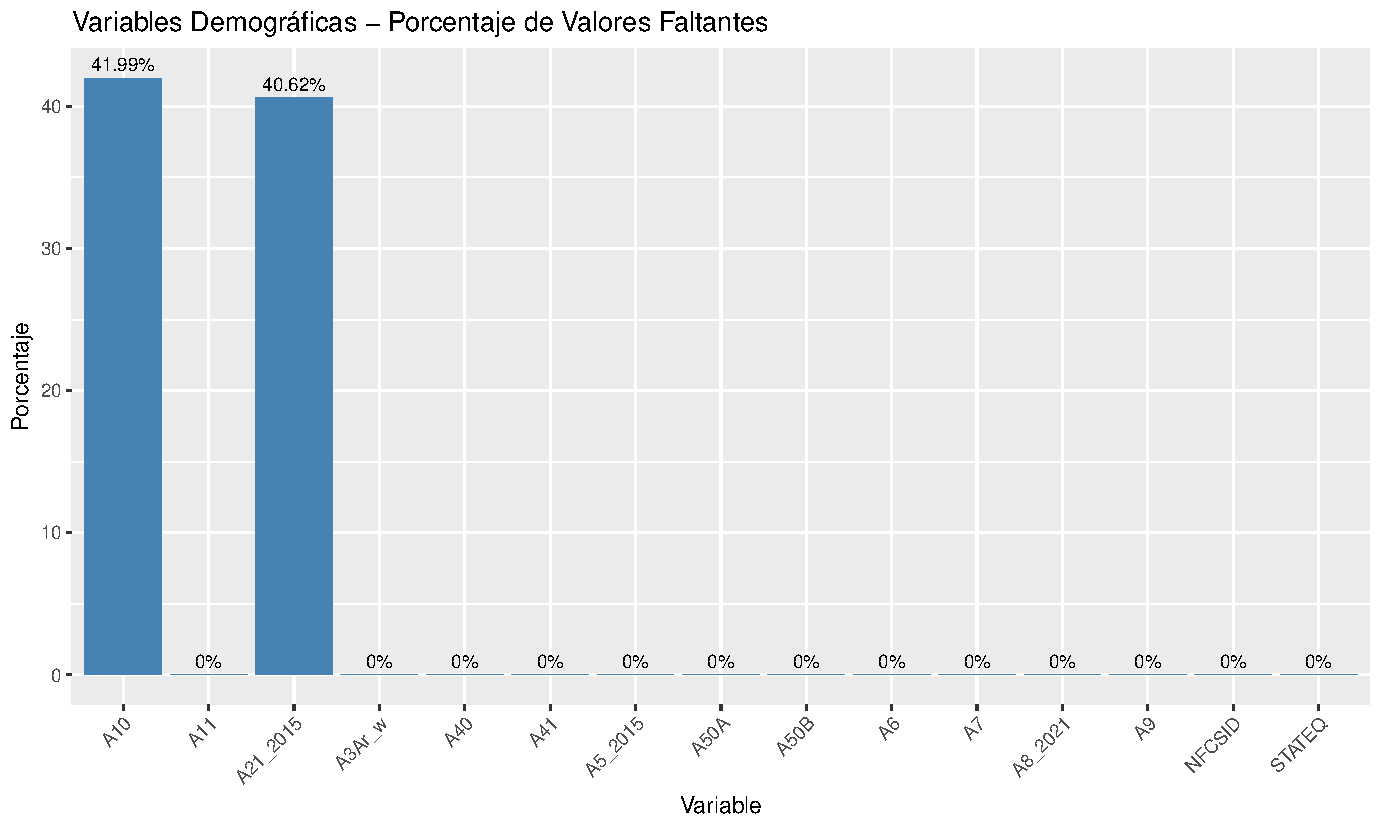
\includegraphics[width=0.8\textwidth]{images/Demographic_Features__Missing_Values.pdf} 
    \caption{Variables Demográficas: valores faltantes}
    \label{fig:demographic_features_missing_values}
\end{figure}

Comenzamos con las variables explicativas demográficas. La figure \ref{fig:demographic_features_missing_values}
recoge el porcentaje de registros que carecen de valor. Como se puede observar, solo dos 
variables explicativas tiene entradas sin definir: (1) \textbf{A10}, con un
\textbf{41.99\%} de valores faltantes y (2) \textbf{A21\_2015}, con un \textbf{40.62\%} de 
valores faltantes. 

Tal y como se puede consultar en la sección \ref{sec:features_description}, la 
primera de las variables corresponde con el estado laboral de la pareja y la segunda informa 
sobre estudiantes a tiempo parcial. Si bien son importantes, dado los elevados porcentajes de
datos faltantes y el elevado numero de otras variables explicativas, se opta por eliminarlas
del estudio.

La figura \ref{fig:capabilities_features_missing_values} presenta el porcentaje de valores 
faltantes para las variables explicativas correspondientes al conjunto de datos de alfabetización
financiera. En este conjunto de datos existen cuatro variables explicativas con valores faltantes:
(1) \textbf{B14}, con un \textbf{4.33\%}, (2) \textbf{C2\_2012}, con un \textbf{62.57\%}, (3) 
\textbf{C5\_2012} con un \textbf{54.04\%} y finalmente (4) \textbf{E7} con un \textbf{41.19\%}. De
nuevo, tal y como se puede comprobar en la sección \ref{sec:features_description} estas variables harían
referencia respectivamente a la inversión en acciones (B14), quién es el promotor de los planes de
pensiones (C2\_2012), si se realizan contribuciones recurrentes al plan de pensiones (C5\_2012) y
la existencia de una hipoteca (E7). En este caso, se eliminarán del conjunto de datos las
variables con elevados porcentaje del valores faltantes y se imputará la variable E14.

\begin{figure}[ht]
    \centering
    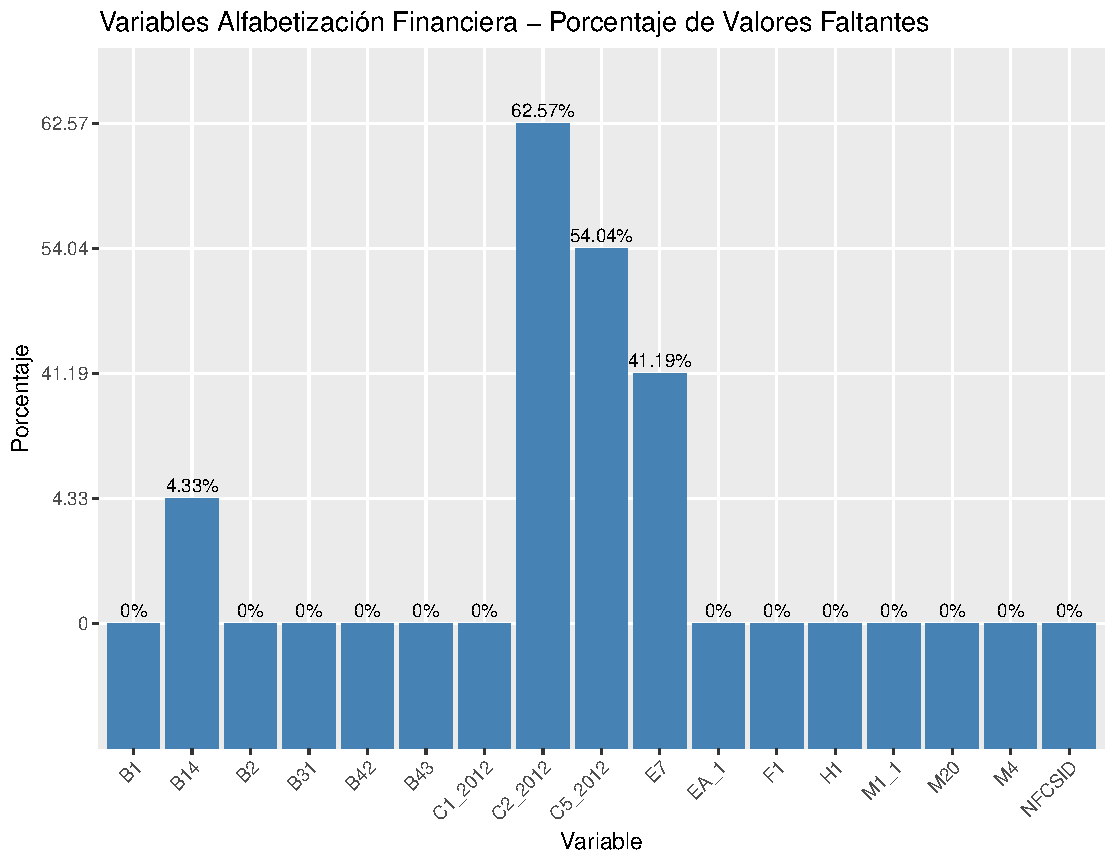
\includegraphics[width=0.8\textwidth]{images/Capabilities_Features__Missing_Values.pdf} 
    \caption{Variables Alfabetización Financiera: valores faltantes}
    \label{fig:capabilities_features_missing_values}
\end{figure}

Por último, la figura \ref{fig:stress_features_missing_values} presenta el porcentaje de valores
faltantes para las variables explicativas correspondientes al conjunto de datos de estrés
financiero. En este caso, existen 10 variables con valores faltantes: (1) \textbf{C10\_2012}, con 
un \textbf{54.04\%}, (2) \textbf{E15\_2015}, con un \textbf{69.3\%}, (3) \textbf{G35}, con un 
\textbf{76.21\%}, (4) \textbf{J6}, con un \textbf{65.6\%}, y el conjunto de variables
\textbf{F2\_1}, \textbf{F2\_2}, \textbf{F2\_3}, \textbf{F2\_4}, \textbf{F2\_5} y \textbf{F2\_6}, 
todas ellas con un porcentaje de valores faltantes de \textbf{21.09\%}. Siguiendo con la 
aproximación anterior, para las cuatro primeras variables, debido al elevado porcentaje de 
valores faltantes se opta por eliminarlas del conjunto de datos. El conjunto de seis variables,
con un quinto de valores faltantes, corresponden todas ellas, a preguntas relacionadas con 
tarjetas de crédito, y de nuevo en este caso, se completarán los valores con imputación.

\begin{figure}[ht]
    \centering
    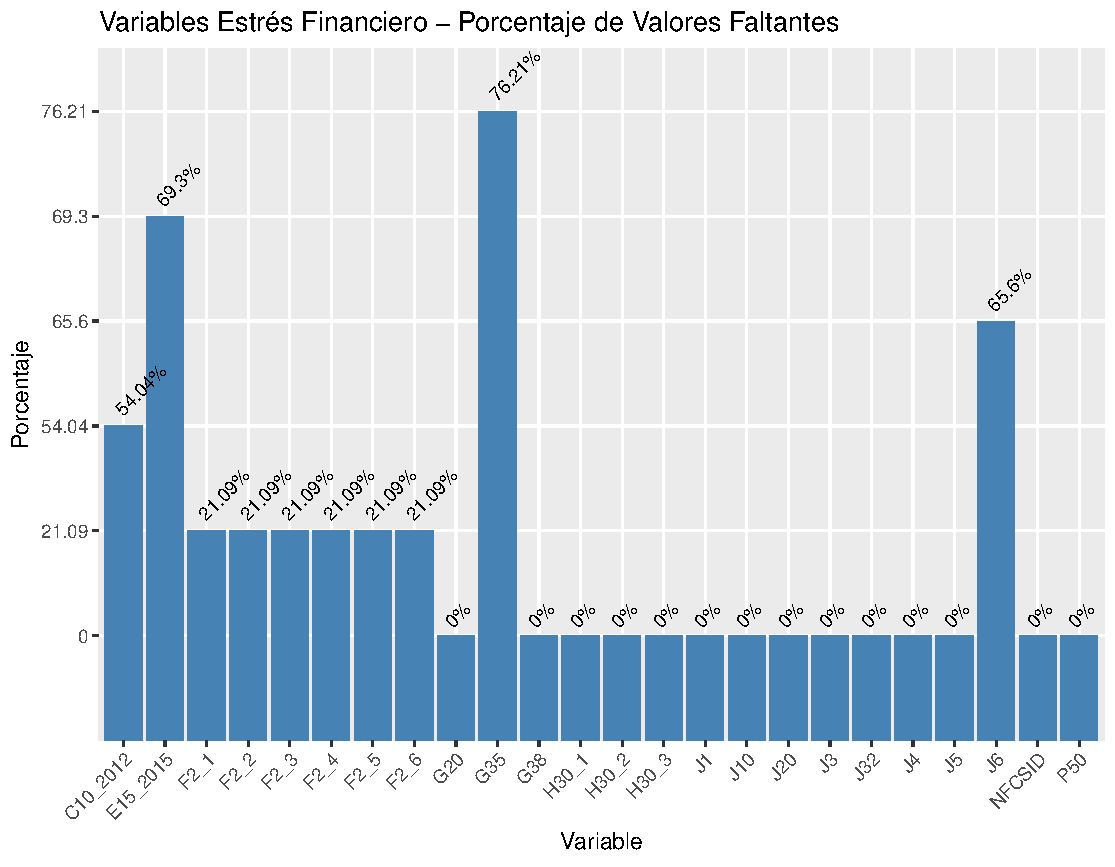
\includegraphics[width=0.8\textwidth]{images/Stress_Features__Missing_Values.pdf} 
    \caption{Variables Estrés Financiero: valores faltantes}
    \label{fig:stress_features_missing_values}
\end{figure}

El proceso de imputación de valores faltantes presenta ciertas limitaciones, derivadas de la
razón que subyace bajo la ausencia de dichos valores. Se podría tratar de un proceso 
puramente aleatorio (\textbf{MCAR}), independiente del valor del resto de variables
explicativas; simplemente, algunos valores se han perdido. 

Alternativamente, la razón que explicaría la ausencia del dato podría depender de las otras 
variables explicativas, pero no del valor ausente (\textbf{MAR}); en nuestra caso podría 
explicar algunos de los valores faltantes. Finalmente los valores faltantes podrían ser una 
respuesta condicionada por el valor en cuestión (\textbf{MNAR}), y por lo tanto sería un 
resultado intencionado y no aleatorio. 

La imputación funcionará mejor en los casos en los que existe algún grado de aleatoriedad \cite{lantz23}, y aunque no es posible discernir a priori la razón
última que explicaría cada uno de los valores faltantes, esta consideración es
necesaria para mantener un escepticismo sano, que eventualmente pueda identificar
situaciones en las que la imputación requiere un análisis mas profundo.
\\

\colorbox{gray!30}{
\begin{minipage}{\textwidth}
\textbf{Librería missForest}\\
  La librería missForest\footnote{https://academic.oup.com/bioinformatics/article/28/1/112/219101}
  corresponde con el estado del arte en R para la imputación de valores
  ausentes. Resulta especialmente recomendada para situaciones en las que se cuenta con variables
  explicativas de tipo categórico, ordinal o numérico, y es capaz por tanto de relaciones complejas,
  proporcionando además un conjunto de datos sobre el proceso.\\

  El proceso seguido sería el siguiente:
  \begin{description}
      \item[Imputación inicial] El procese se inicial realizando un imputación, que en el caso  
      de variables categóricas corresponde con el valor mas frecuente.
      \item[Revisión] Se revisan los valores asignados a cada registro y se analizando el valor
      que presentan el resto de variables del registro, se mejora la imputación inicial, utilizando
      un \textit{random forest}.
      \item[Iteración] El proceso se repite hasta alcanzar el número máximo de iteraciones o se 
      cumple un criterio definido de finalización.
  \end{description}
\end{minipage}
}
\\
A modo ilustrativo se recoge la distribución de los distintos niveles, comparando los valores
originales con las imputaciones. Como se aprecia en la figura \ref{fig:Analysis_MV_B14}, no 
existe una diferencia apreciable entre los valores originales y los imputados, lo que es consistente con el reducido porcentaje de valores faltantes que se daban en la variable B14.

\begin{figure}[ht]
    \centering
    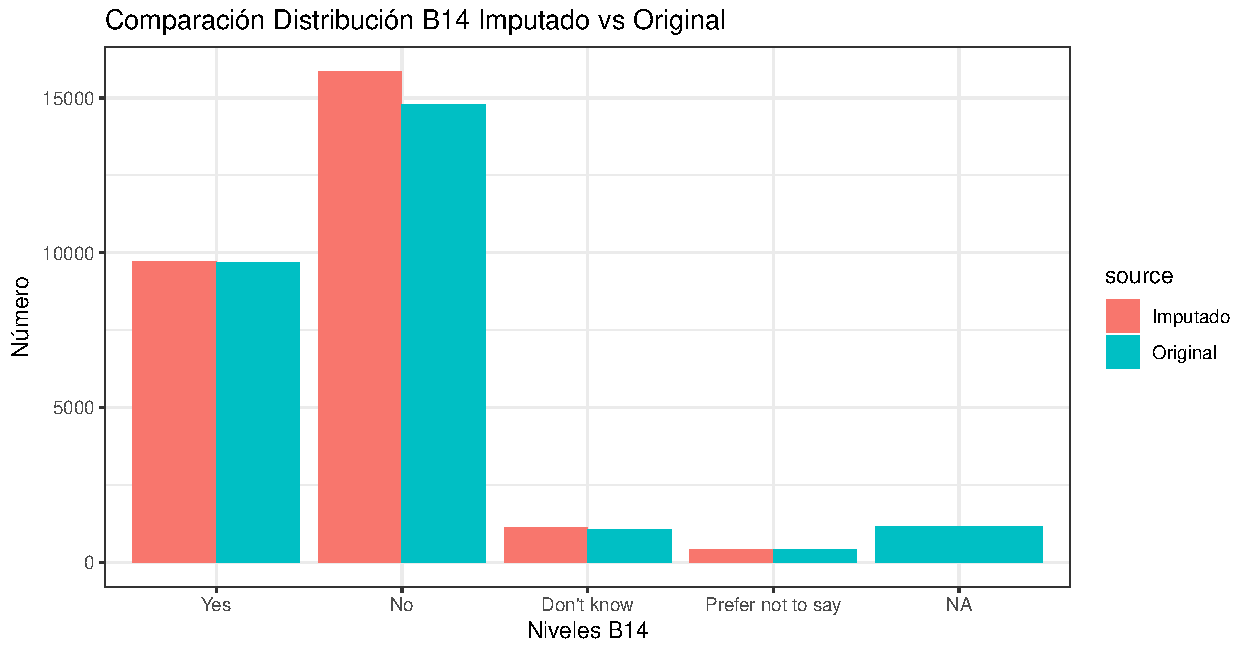
\includegraphics[width=0.8\textwidth]{images/Analysis_MV_B14.pdf} 
    \caption{Variables Alfabetización Financiera: valores faltantes}
    \label{fig:Analysis_MV_B14}
\end{figure}

Seguidamente se presenta las mismas figuras resumen para las variables con valores faltantes 
correspondientes al conjunto de datos representando el estrés financiero. Como se aprecia, el 
resultado es muy similar para todas las variables ya que todas ellas presentaban un 
porcentaje similar de valores faltantes. Las diferencias apreciables son debidas al las 
diferencias entre el resto de variables, que hacen que el algoritmo de \textit{random forest} 
resulte en imputaciones ligeramente distintas.

\begin{figure}[ht]
    \centering
    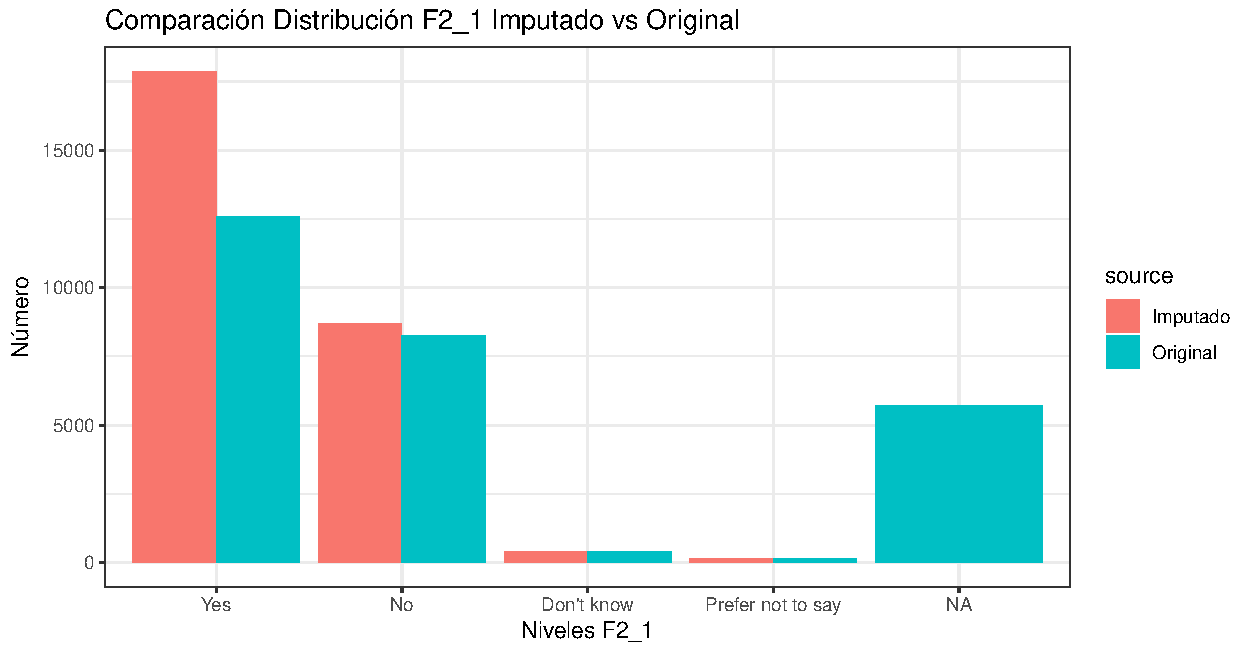
\includegraphics[width=0.8\textwidth]{images/Analysis_MV_F2_1.pdf} 
    \caption{Análisis F2\_1 valores Imputados vs Originales}
    \label{fig:Analysis_MV_F2_1}
\end{figure}

\begin{figure}[ht]
    \centering
    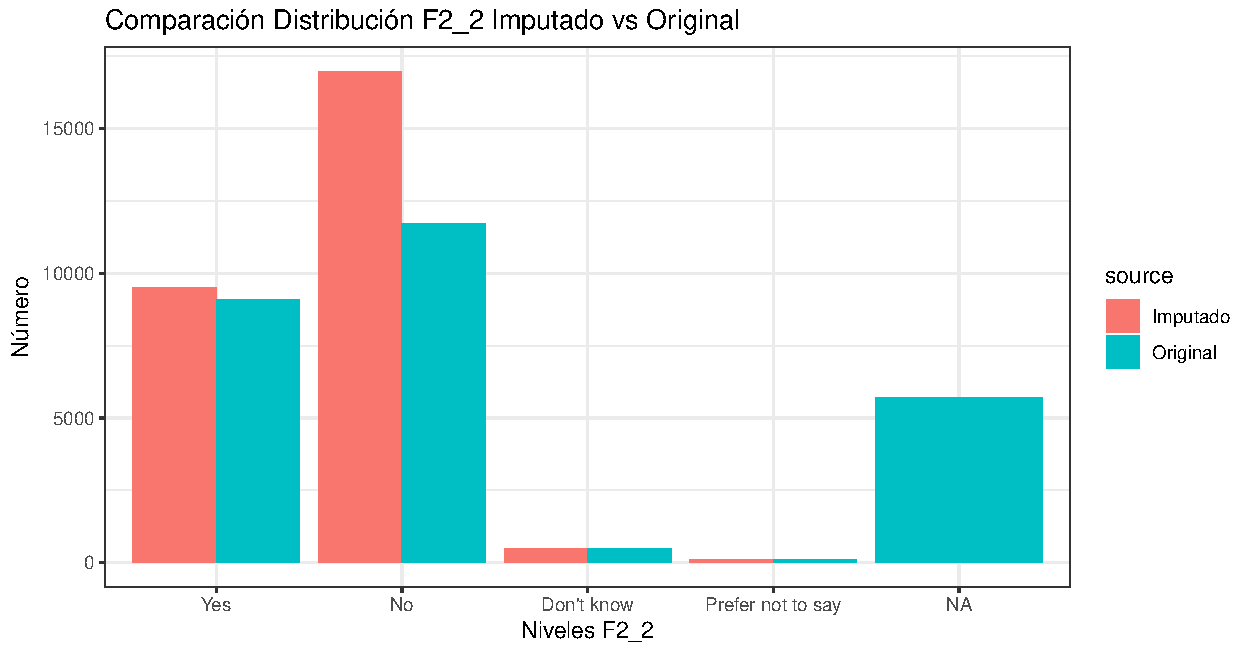
\includegraphics[width=0.8\textwidth]{images/Analysis_MV_F2_2.pdf} 
    \caption{Análisis F2\_2 valores Imputados vs Originales}
    \label{fig:Analysis_MV_F2_2}
\end{figure}

\begin{figure}[ht]
    \centering
    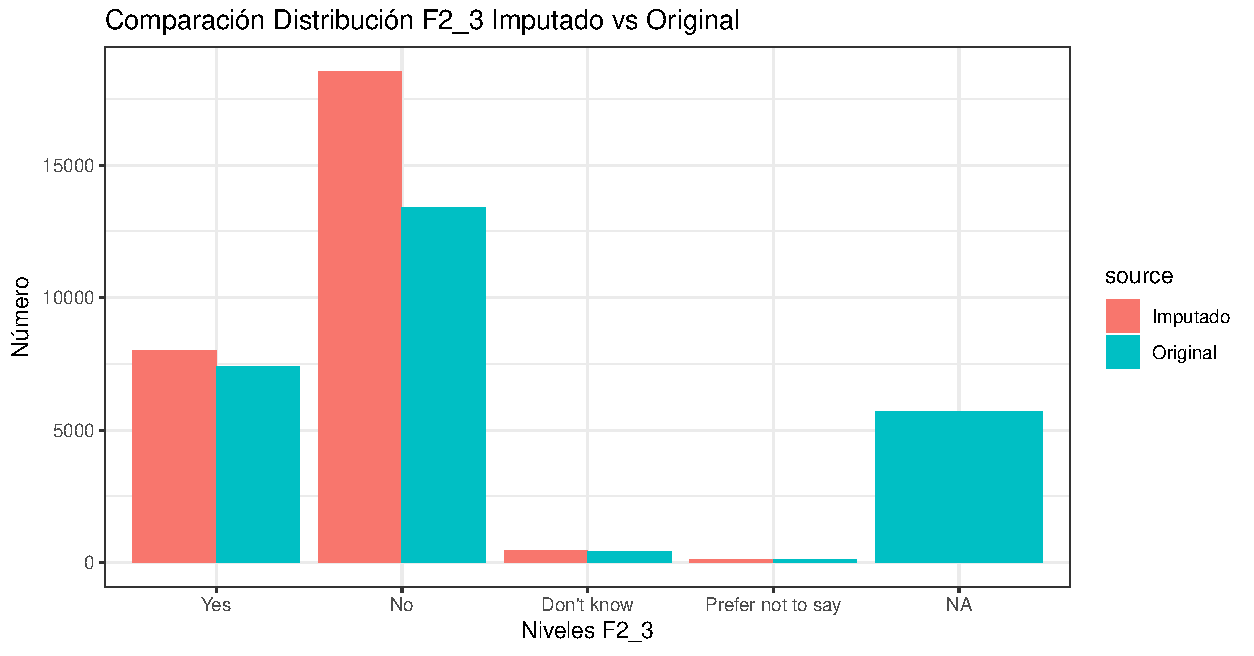
\includegraphics[width=0.8\textwidth]{images/Analysis_MV_F2_3.pdf} 
    \caption{Análisis F2\_3 valores Imputados vs Originales}
    \label{fig:Analysis_MV_F2_3}
\end{figure}

\begin{figure}[ht]
    \centering
    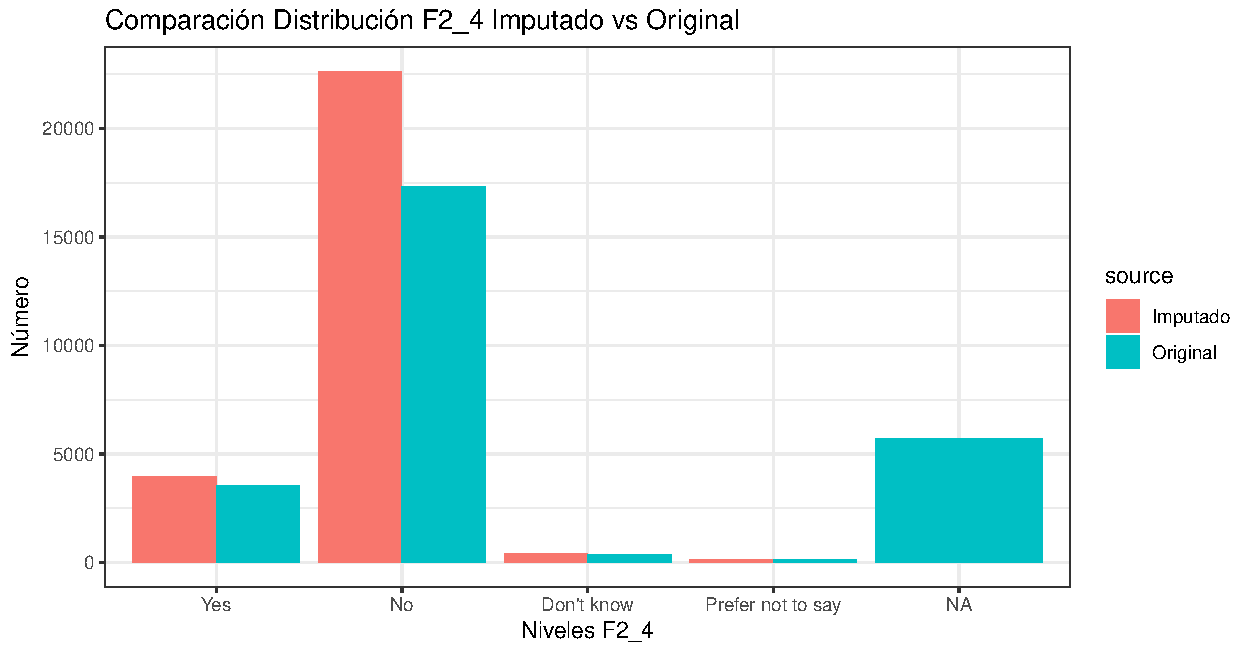
\includegraphics[width=0.8\textwidth]{images/Analysis_MV_F2_4.pdf} 
    \caption{Análisis F2\_4 valores Imputados vs Originales}
    \label{fig:Analysis_MV_F2_4}
\end{figure}

\begin{figure}[ht]
    \centering
    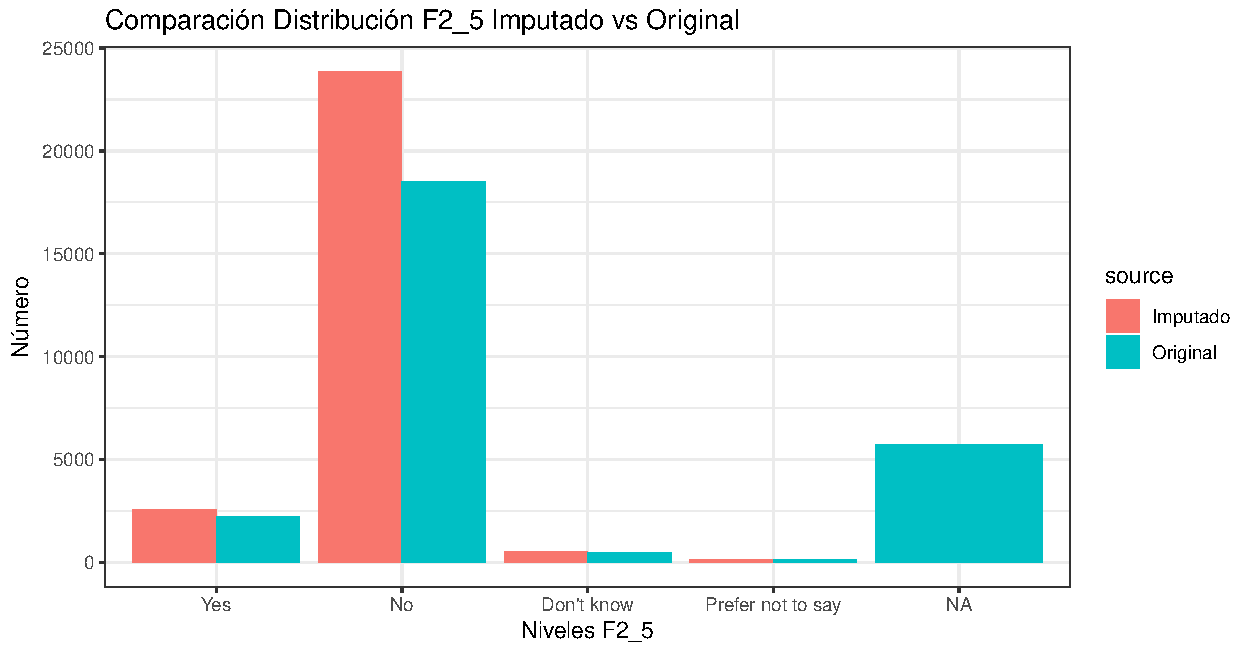
\includegraphics[width=0.8\textwidth]{images/Analysis_MV_F2_5.pdf} 
    \caption{Análisis F2\_5 valores Imputados vs Originales}
    \label{fig:Analysis_MV_F2_5}
\end{figure}

\begin{figure}[ht]
    \centering
    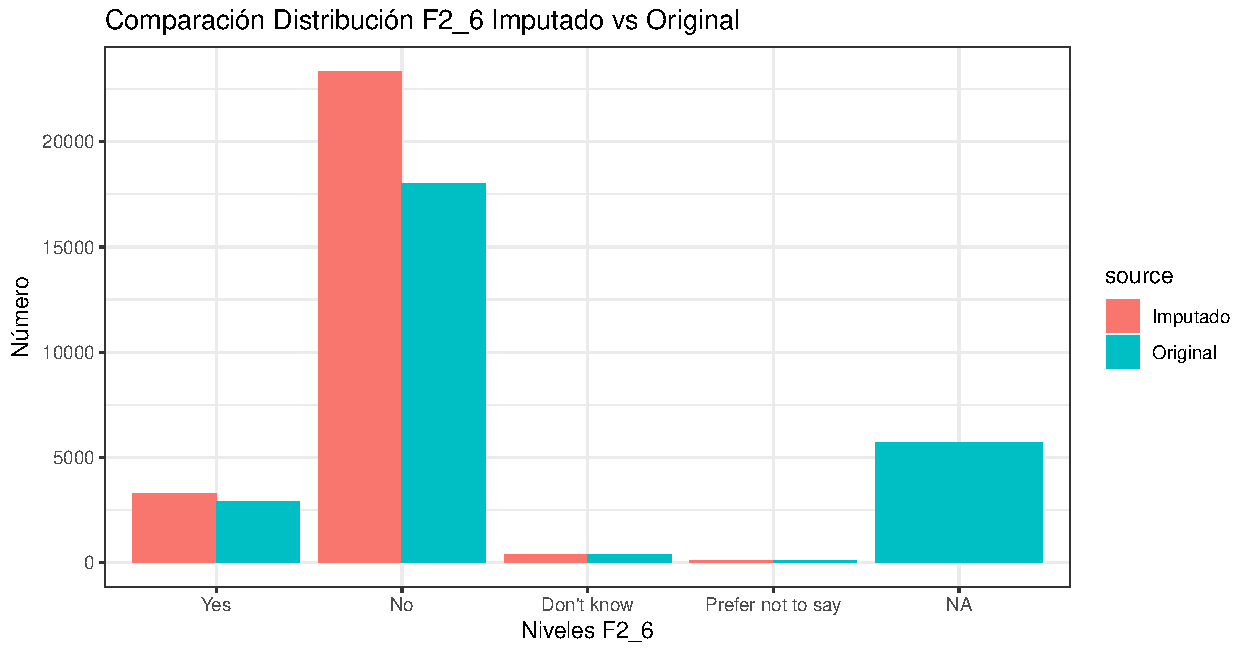
\includegraphics[width=0.8\textwidth]{images/Analysis_MV_F2_6.pdf} 
    \caption{Análisis F2\_6 valores Imputados vs Originales}
    \label{fig:Analysis_MV_F2_6}
\end{figure}

\subsection{Codificación de Variables Categóricas}
El conjunto de datos NFCS 2021 esta formado por variables categóricas, nominales, que
representan las respuestas de los participantes en el estudio a preguntas con un
conjunto de opciones. El procesamiento requiere la codificación de estas variables
y en este caso se utiliza el código denominado \textit{one-hot}. 

Para cada factor, este código introduce una nueva variable binaria por cada uno de los
niveles. El resultado es la explosión dimensional del conjunto de datos y el carácter
disperso de la matriz que los representa. Desde el punto de vista de programación, 
el proceso es extremadamente sencillo, ya que utilizando la librería \textit{mltools}, se
reduce a una instrucción.

En la investigación que nos ocupa, y más tras el tratamiento de los valores faltantes, los
conjuntos de datos no son especialmente grandes, por lo que el impacto de la codificación
\textit{one-hot} no será importante; en particular el conjunto de datos demográficos  para
de XX a YY dimensiones, el conjunto de datos de alfabetización financiera pasa de XX a YY
dimensiones y el conjunto de datos de estrés financiero para de XX a YY dimensiones.

\subsection{Taxonomías}
\label{sec:sub:clustering}
Una vez preparados los conjuntos de datos se realizará una taxonomía siguiendo un proceso
jerárquico, que comenzará con la introducción de una taxonomía del estrés financiero, para
continuar con una taxonomía de la alfabetización financieras y finalmente
se cruzarán esos datos con los demográficos para clasificar la población en conjunto.

Una vez obtenidas las clasificaciones o taxonomías anteriores, y tras etiquetar los conjuntos
adecuadamente se desarrollarán, utilizando un aprendizaje supervisado, clasificadores que 
permitan partiendo de los datos demográficos o de alfabetización financiera determinar el 
nivel de estrés financiero, ya sea para recomendar medidas de alfabetización financiera 
paliativas o de prevención.



%%\section{Análisis y evaluación de los resultados obtenidos}
%%\section{Conclusiones}
%%\section{Anexo: código}
\section{Variables Explicativas: listado y descripción}
\label{sec:features_description}
El presente apéndice recoge las descripciones de las variables explicativas, todas ellas categóricas, 
que se han utilizado en la investigación. Para información adicional sobre el conjunto de datos 
consúltese la referencia \cite{NFCS01}.

\begin{table}
\centering
\footnotesize
\begin{tabular}{>{\RaggedRight\hspace{0pt}}m{2cm} >{\RaggedRight\hspace{0pt}}m{11cm}}
\toprule
\textbf{Variable} & \textbf{Descripción}\\
\midrule
NFCSID & Respondent ID \\
STATEQ & State \\
A50A & [GENDER (non-binary randomly assigned)]\\
A3Ar\_w & Age group \\
A50B & [GENDER/AGE NET (non-binary randomly assigned)] \\
A5\_2015 & What was the highest level of education that you completed? [2015 codes] \\
A6 & What is your marital status?\\
A7 & Which of the following describes your current living arrangements?\\
A11 & How many children do you have who are financially dependent on you [or your spouse/partner]?\\
A8\_2021 & What is your [household's] approximate annual income, including wages, tips, investment income, public assistance, income from retirement plans, etc.? [2021 codes] \\
A9 & Which of the following best describes your current employment or work status?  \\
A40 & [In addition to your main employment, did you also do other/Did you do any] work for pay in the past 12 months?\\
A10 & Which of the following best describes your [spouse's/partner's] current employment or work status? \\
A21\_2015 & Are you a part-time student taking courses for credit? [2015 base]\\
A41 & What was the highest level of education completed by the person or any of the people who raised you?\\
\bottomrule
\end{tabular}
\caption{Demografía: Variables Explicativas}
\label{table:demographics_features}
\end{table}

\begin{table}
\centering
\footnotesize
\begin{tabular}{>{\RaggedRight\hspace{0pt}}m{2cm} >{\RaggedRight\hspace{0pt}}m{11cm}}
\toprule
\textbf{Variable} & \textbf{Descripción} \\
\midrule
\textbf{NFCSID} & Respondent ID\\
\textbf{B1} & Do you [Does yourhousehold] have a checking account?  \\
\textbf{B2} & Do you [Does your household] have a savings account, money market account, or CDs?\\
\textbf{B31} & How often do you use your mobile phone to pay for a product or service in person at a store, gas station, or restaurant (e.g., by waving/tapping your mobile phone over a sensor at checkout, scanning a barcode or QR code using your mobile phone, or using so\\
\textbf{B42} & How often do you use your mobile phone to transfer money to another person?\\
\textbf{B43} & How often do you use websites or apps to help with financial tasks such as budgeting, saving, or credit management (e.g., GoodBudget, Mint, Credit Karma, etc.)? Please do not include websites or apps for making payments or money transfers.\\
\textbf{C1\_2012} & Do you [or your spouse/partner] have any retirement plans through a current or previous employer, like a pension plan, [a Thrift Savings Plan (TSP),] or a 401(k)? [2012 base] \\
\textbf{C2\_2012} & Were these plans provided by your employer or your [spouse's/partner's] employer, or both? [2012 base] \\
\textbf{C5\_2012} & Do you [or your spouse/partner] regularly contribute to a retirement account like a [Thrift Savings Plan (TSP),] 401(k) or IRA? [2012 base]\\
\textbf{B14} & Not including retirement accounts, do you [does your household] have any investments in stocks, bonds, mutual funds, or other securities? \\
\textbf{EA\_1} & Do you [or your spouse/partner] currently own your home?\\
\textbf{E7} & Do you currently have any mortgages on your home?\\
\textbf{F1} & How many credit cards do you have?\\
\textbf{H1} & Are you covered by health insurance?\\
\textbf{M1\_1} & How strongly do you agree or disagree with the following statements? - I am good at dealing with day-to-day financial matters, such as checking accounts, credit and debit cards, and tracking expenses \\
\textbf{M4} & On a scale from 1 to 7, where 1 means very low and 7 means very high, how would you assess your overall financial knowledge? \\
\textbf{M20} & Was financial education offered by a school or college you attended, or a workplace where you were employed?\\
\bottomrule
\end{tabular}
\caption{Alfabetización Financiera: Variables Explicativas}
\label{table:capabilities_features}
\end{table}

\begin{table}
\centering
\footnotesize
\begin{tabular}{>{\RaggedRight\hspace{0pt}}m{2cm} >{\RaggedRight\hspace{0pt}}m{11cm}}
\toprule
\textbf{Variable} & \textbf{Descripción}\\
\midrule
\textbf{NFCSID} & Respondent ID \\
\textbf{J1} & Overall, thinking of your assets, debts and savings, how satisfied are you with your current personal financial condition?  \\
\textbf{J3} & Over the past year, would you say your [household's] spending was less than, more than, or about equal to your [household's] income?  \\
\textbf{J4} & In a typical month, how difficult is it for you to cover your expenses and pay all your bills?  \\
\textbf{J5} & Have you set aside emergency or rainy day funds that would cover your expenses for 3 months, in case of sickness, job loss, economic downturn, or other emergencies?  \\
\textbf{J6} & Are you setting aside any money for your children's college education?\\
\textbf{J10} & In the past 12 months, have you [has your household] experienced a large drop in income which you did not expect? \\
\textbf{J20} & How confident are you that you could come up with \$2,000 if an unexpected need arose within the next month?  \\
\textbf{J32} & How would you rate your current credit record? \\
\textbf{C10\_2012} & In the last 12 months, have you [or your spouse/partner] taken a loan from your retirement account(s)? [2012 base]  \\
\textbf{E15\_2015} & How many times have you been late with your mortgage payments in the past 12 months? [2015 time frame]  \\
\textbf{F2\_1} & In the past 12 months, which of the following describes your experience with credit cards? - I always paid my credit cards in full  \\
\textbf{F2\_2} & In the past 12 months, which of the following describes your experience with credit cards? - In some months, I carried over a balance and was charged interest \\
\textbf{F2\_3} & In the past 12 months, which of the following describes your experience with credit cards? - In some months, I paid the minimum payment only \\
\textbf{F2\_4} & In the past 12 months, which of the following describes your experience with credit cards? - In some months, I was charged a late fee for late payment  \\
\textbf{F2\_5} & In the past 12 months, which of the following describes your experience with credit cards? - In some months, I was charged an over the limit fee for exceeding my credit line  \\
\textbf{F2\_6} & In the past 12 months, which of the following describes your experience with credit cards? - In some months, I used the cards for a cash advance  \\
\textbf{P50} & At any time in your adult life (18 and older), did your parents or grandparents pay for an expense of yours that was \$10,000 or more?  \\
\textbf{G20} & Do you currently have any unpaid bills from a health care or medical service provider (e.g., a hospital, a doctor's office, or a testing lab) that are past due?  \\
\textbf{G35} & How many times have you been late with a student loan payment in the past 12 months? \\
\textbf{G38} & Have you been contacted by a debt collection agency in the past 12 months? \\
\textbf{H30\_1} & In the last 12 months, was there any time when you… - Did NOT fill a prescription for medicine because of the cost  \\
\textbf{H30\_2} & In the last 12 months, was there any time when you… - SKIPPED a medical test, treatment or follow-up recommended by a doctor because of the cost  \\
\textbf{H30\_3} & In the last 12 months, was there any time when you… - Had a medical problem but DID NOT go to a doctor or clinic because of the cost  \\
\bottomrule
\end{tabular}
\caption{Estrés Financiero: Variables Explicativas}
\label{table:stress_features}
\end{table}
\newpage
\printbibliography 
\end{document}
